%%%%%%%%%%%%%%%%%%%%%%%%%%%%%%%%%%%%%%%%%%%%%%%%%%%%%%%%%%%%%%%%%%%%%%
% LaTeX Template: Designer's CV
%
% Source: http://www.howtotex.com
% 
% Feel free to distribute this example, but please keep the referral
% to HowToTeX.com
% 
% Date: March 2012
%
% Modified by Lim Lian Tze to support multiple pages using fix provided at
% http://www.howtotex.com/templates/creating-a-designers-cv-in-latex/
% Date: November 2014
%%%%%%%%%%%%%%%%%%%%%%%%%%%%%%%%%%%%%%%%%%%%%%%%%%%%%%%%%%%%%%%%%%%%%%
% How to use writeLaTeX: 
%
% You edit the source code here on the left, and the preview on the
% right shows you the result within a few seconds.
%
% Bookmark this page and share the URL with your co-authors. They can
% edit at the same time!
%
% You can upload figures, bibliographies, custom classes and
% styles using the files menu.
%
% If you're new to LaTeX, the wikibook is a great place to start:
% http://en.wikibooks.org/wiki/LaTeX
%
%%%%%%%%%%%%%%%%%%%%%%%%%%%%%%%%%%%%%%%%%%%%%%%%%%%%%%%%%%%%%%%%%%%%%%

%%%%%%%%%%%%%%%%%%%%%%%%%%%%%%%%%%%%%
% Document properties and packages
%%%%%%%%%%%%%%%%%%%%%%%%%%%%%%%%%%%%%
\documentclass[a4paper,12pt,final]{memoir}

% misc
\renewcommand{\familydefault}{bch}	% font
\pagestyle{empty}					% no pagenumbering
\setlength{\parindent}{0pt}			% no paragraph indentation


% required packages (add your own)
\usepackage{flowfram}										% column layout
\usepackage[top=1cm,left=1cm,right=1cm,bottom=1cm]{geometry}% margins
\usepackage{graphicx}										% figures
\usepackage{url}											% URLs
\usepackage[usenames,dvipsnames]{xcolor}					% color
\usepackage{multicol}										% columns env.
	\setlength{\multicolsep}{0pt}
\usepackage{paralist}										% compact lists
\usepackage{tikz}

%%%%%%%%%%%%%%%%%%%%%%%%%%%%%%%%%%%%%
% Create column layout
%%%%%%%%%%%%%%%%%%%%%%%%%%%%%%%%%%%%%
% define length commands
\setlength{\vcolumnsep}{\baselineskip}
\setlength{\columnsep}{\vcolumnsep}

% left frame
\newflowframe{0.3\textwidth}{\textheight}{0pt}{0pt}[left]
	\newlength{\LeftMainSep}
	\setlength{\LeftMainSep}{0.22\textwidth}
	\addtolength{\LeftMainSep}{1\columnsep}
 
% small static frame for the vertical line
\newstaticframe{1.5pt}{\textheight}{\LeftMainSep}{0pt}
 
% content of the static frame
\begin{staticcontents}{1}
\hfill
\tikz{%
	\draw[loosely dotted,color=RoyalBlue,line width=1.5pt,yshift=0]
	(0,0) -- (0,\textheight);}%
\hfill\mbox{}
\end{staticcontents}
 
% right frame
\addtolength{\LeftMainSep}{1.5pt}
\addtolength{\LeftMainSep}{1\columnsep}
\newflowframe{0.7\textwidth}{\textheight}{\LeftMainSep}{0pt}[main01]


%%%%%%%%%%%%%%%%%%%%%%%%%%%%%%%%%%%%%
% define macros (for convenience)
%%%%%%%%%%%%%%%%%%%%%%%%%%%%%%%%%%%%%
\newcommand{\Sep}{\vspace{1.5em}}
\newcommand{\SmallSep}{\vspace{0.5em}}

\newenvironment{AboutMe}
	{\ignorespaces\textbf{\color{RoyalBlue} About me}}
	{\Sep\ignorespacesafterend}
	
\newcommand{\CVSection}[1]
	{\Large\textbf{#1}\par
	\SmallSep\normalsize\normalfont}

\newcommand{\CVItem}[1]
	{\textbf{\color{RoyalBlue} #1}}


%%%%%%%%%%%%%%%%%%%%%%%%%%%%%%%%%%%%%
% Begin document
%%%%%%%%%%%%%%%%%%%%%%%%%%%%%%%%%%%%%
\begin{document}

% Left frame
%%%%%%%%%%%%%%%%%%%%
%
% Upload your own photo using the files menu
\begin{figure}
	%\hfill
	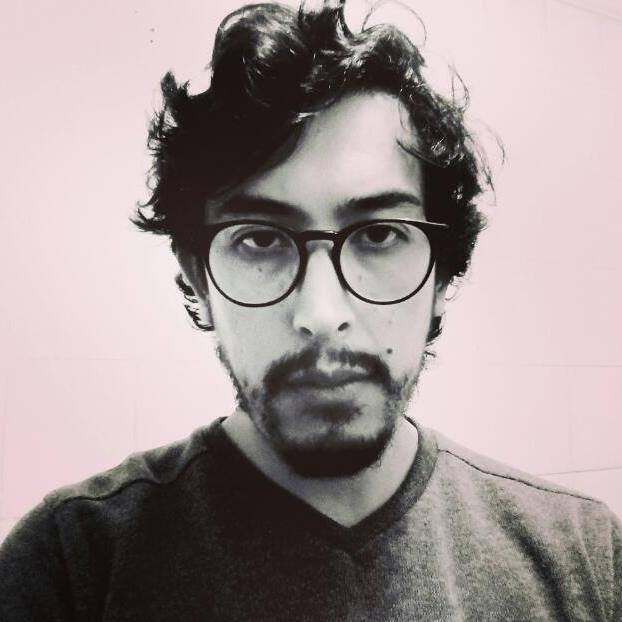
\includegraphics[width=0.75\columnwidth]{my-pic.jpg}
	\vspace{-2cm}
\end{figure}

\begin{flushleft}\small
    \vspace{10mm}
    \textbf{Contact Details}\\
    \vspace{1mm}
	Pablo Ibieta\\
	\vspace{1mm}
	CPF 236.705.918-40 \\
	\vspace{1mm}
    
\includegraphics[width=0.07\columnwidth]{gmail_icon.png} ibieta.pablo@gmail.com \\
    \vspace{1mm}
    
\includegraphics[width=0.08\columnwidth]{usp_icon.png} pibieta@if.usp.br \\
    
\includegraphics[width=0.07\columnwidth]{cellphone_icon.png} (+55) 11 959 360 119 \\	
	\vspace{4mm}
	\textbf{Work Address}\\
	\vspace{1mm}
	Rua do Mat\~ao Travessa R\\
	\vspace{1mm}
	Nr. 187, Off. 331 \\
	\vspace{1mm}
	CEP 05508-090\\
	\vspace{1mm}
	S\~{a}o Paulo, Brazil.\\
	\vspace{4mm}
	\textbf{Personal Address}\\
	\vspace{1mm}
	Rua Frei In\'{a}cio \\
	\vspace{1mm}
	da Conceição 237, Apto 6 \\
	\vspace{1mm}
	CEP 05362-040 \\
	\vspace{1mm}
	S\~{a}o Paulo, Brazil.\\
	\vspace{4mm}
	\textbf{Details and Publications}\\
	\vspace{1mm}
	Curriculo Lattes \\
	\vspace{1mm}
	https://bit.ly/2CXGU8i\\
	\vspace{1mm}
    
\includegraphics[width=0.07\columnwidth]{in_icon.png} /in/pibieta \\
    \vspace{1mm}
    
\includegraphics[width=0.07\columnwidth]{git.jpeg} /pibieta \\
    \vspace{1mm}
    \vspace{4mm}
	\textbf{Languages}\\
	\vspace{1mm}
	Spanish: Mother tongue\\
	\vspace{1mm}
	English: Fluent\\
	\vspace{1mm}
	Portuguese: Fluent\\
	\vspace{1mm}
	French: Basic
	\vspace{1mm}
\end{flushleft}\normalsize


\framebreak



% Right frame
%%%%%%%%%%%%%%%%%%%%
\Huge\bfseries {\color{RoyalBlue} Pablo Ibieta} \\
\Large\bfseries Physicist / Data Scientist \\

\normalsize\normalfont

% About me
\begin{AboutMe}
Since 2012, I have worked as a scientific researcher in the area of Mathematical Physics. During this period, I have acquired advanced mathematical knowledge and learned several computational skills concerning data analysis. This involves the manipulation and interpretation of data, the use of statistical tools to compare data to models and the computation of experimental predictions using simulations. In order to complement these skills, basically oriented to industry applications, currently I am focused on the study and development of Python based Data Science and Machine Learning tools. 
\end{AboutMe}
 
% Experience
\CVSection{Experience}
\CVItem{Sep 2012 - present}\\
Junior Researcher and Teaching Assistant,  Instituto de F\'{i}sica, Universidade de S\~{a}o Paulo 
(USP). S\~{a}o Paulo, Brazil. Project: \emph{Topological Quantum Field Theories and Topological Phases of Matter} (5 PUBS).
\SmallSep


\CVItem{Jan 2018}\\
Visiting Professor, Universidad Mayor de San Andr\'{e}s, Physics Department. La Paz, Bolivia. Project: \emph{Taught the \textbf{Group Theory and Physics} course at the Summer School}
\SmallSep

\CVItem{Sep 2005 - Feb 2010}\\
Junior Researcher and Teaching Assistant. Institute for Theoretical Physics,
Universidad Mayor de San Andr\'{e}s, Physics Department. La Paz, Bolivia. Project: \emph{Performed research on Loop Quantum Gravity} (1 PUB).
%\SmallSep

\Sep

% Education
\CVSection{Education}
\CVItem{2015 - 2019}\\
Ph. D. in Physics, Universidade de S\~{a}o Paulo (USP).\\ 
S\~{a}o Paulo, Brazil. Thesis:  \emph{Topological entanglement entropy and Area Law in Higher Gauge Theories.} 
\SmallSep

\CVItem{2012 - 2015}\\
M. Sc. in Physics, Universidade de S'\~{a}o Paulo (USP)\\
S\~{a}o Paulo, Brazil. Thesis: \emph{Gauge and Matter Fields on Lattice}
\SmallSep

\CVItem{2004 - 2010}\\
Bachelor in Physics, Universidad Mayor de San Andr\'{e}s (UMSA).\\
La Paz, Bolivia. \emph{Entropy of a Rotating Black Hole in LQG}.

\Sep

\CVSection{Skills}

% Skills

\CVItem{Team Work}\\
Teacher and coordinator of three undergraduate physics courses at USP.\\
Teaching assistant of several courses at UMSA and USP.
\SmallSep

\CVItem{Software Development}\\
Senior experience using Python, R, C, C\texttt{++}, Mathematica and MATLAB.\\
Familiar with libraries Tensorflow, Keras, sklearn and XGBoost. 

% References

%\CVSection{References}

%References upon request.

%%%%%%%%%%%%%%%%%%%%%%%%%%%%%%%%%%%%%
% End document
%%%%%%%%%%%%%%%%%%%%%%%%%%%%%%%%%%%%%
\end{document}